% !TEX program = xelatex
\documentclass[a4paper,12pt]{article}

\usepackage{geometry}
\geometry{a4paper, left=25mm, right=15mm, top=20mm, bottom=20mm}

\usepackage{polyglossia}
\setdefaultlanguage{ukrainian}
\setotherlanguage{english}

\usepackage{fontspec}
\setmainfont{Times New Roman}
\setmonofont{PT Mono}[Scale=0.85]
\newfontfamily\cyrillicfonttt{PT Mono}[Scale=0.85]

\usepackage{graphicx}
\usepackage{float}
\usepackage{hyperref}
\usepackage{listings}
\usepackage{booktabs}
\usepackage{tabularx}
\newcolumntype{L}{>{\raggedright\arraybackslash}X}
\usepackage{fancyhdr}
\usepackage{amsmath}

\lstdefinelanguage{Go}{
    keywords={break,default,func,interface,select,case,defer,go,map,struct,
             chan,else,goto,package,switch,const,fallthrough,if,range,type,
             continue,for,import,return,var,nil,true,false},
    keywordstyle=\bfseries,
    sensitive=true,
    comment=[l]{//},
    morecomment=[s]{/*}{*/},
    string=[b]",
}

\lstset{
    language=Go,
    basicstyle=\ttfamily\footnotesize,
    breaklines=true,
    columns=fullflexible,
    showstringspaces=false,
    numbers=left,
    numberstyle=\tiny,
    stepnumber=1,
    numbersep=8pt,
}

\setlength{\headheight}{14pt}
\pagestyle{fancy}
\fancyhf{}
\fancyhead[L]{\small Лабораторний проєкт~4}
\fancyhead[R]{\small TCP sort client/server}
\fancyfoot[C]{\thepage}

\begin{document}

\begin{titlepage}
    \thispagestyle{empty}
    \begin{center}
        \textbf{Київський національний університет імені Тараса Шевченка}\\
        \textbf{Факультет комп'ютерних наук та кібернетики}
    \end{center}

    \vspace{4cm}

    \begin{center}
        \textbf{\Large ЗВІТ}\\
        \vspace{0.5cm}
        \textbf{\large до лабораторного проєкту №\,4}\\
        \vspace{0.5cm}
        з дисципліни \textit{«Операційні системи»}\\
        \vspace{0.7cm}
        \textbf{Тема: Клієнт--серверне сортування масиву}
    \end{center}

    \vfill

    \begin{flushright}
        Виконав:\\
        Кіщук Ярослав Ярославович
    \end{flushright}

    \vspace{1.5cm}

    \begin{center}
        Київ --- 2026
    \end{center}
\end{titlepage}

\section{Постановка задачі}

Згідно з умовою лабораторного проєкту~4:

\begin{itemize}
    \item Написати програму-сервер і програму-клієнт для розв'язання задачі
    сортування масиву. Клієнт формує масив і відправляє на сервер; сервер
    сортує і відправляє відсортований масив на клієнт.
    \item На клієнті фіксувати час початку відправлення масиву і час
    завершення отримання результатів.
    \item Виконати експеримент 100~разів і визначити середній показник
    швидкості роботи мережного порту.
    \item Кількість елементів --- 10\,000; метод сортування --- на вибір
    (у цій роботі --- \textbf{QuickSort}, $O(n \log n)$ у середньому).
\end{itemize}

\section{Протокол і архітектура}

Транспорт --- TCP (\texttt{127.0.0.1:9504}, loopback). Бінарний формат
повідомлення:

\begin{center}
\begin{tabular}{ll}
\toprule
Поле & Розмір \\
\midrule
\texttt{N} & 4 байти, \texttt{uint32} little-endian \\
\texttt{data} & $N \times 4$ байти (\texttt{int32}) \\
\bottomrule
\end{tabular}
\end{center}

Обсяг одного round-trip (запит + відповідь):
$2 \times (4 + 10000 \times 4) = 80\,008$~байт.

Середня швидкість порту:
\[
V = \frac{2 \cdot (4 + N \cdot 4) \cdot 8}{T_{\mathrm{avg}}} \quad \text{(Мбіт/с)},
\]
де $T_{\mathrm{avg}}$ --- середній час від початку відправлення до завершення
читання відповіді на клієнті.

\section{Код сервера}

\lstinputlisting[caption={\texttt{cmd/server/main.go}}]{../cmd/server/main.go}

\lstinputlisting[caption={\texttt{internal/protocol/array.go}}]{../internal/protocol/array.go}

\lstinputlisting[caption={\texttt{internal/sort/quicksort.go}}]{../internal/sort/quicksort.go}

\section{Код клієнта}

\lstinputlisting[caption={\texttt{cmd/client/main.go}}]{../cmd/client/main.go}

\section{Результати випробувань}

Платформа: macOS, Apple Silicon, loopback TCP.
Експеримент: \texttt{./examples/run\_experiment.sh} (100~прогонів,
\texttt{seed=42}).

\begin{table}[H]
\centering
\caption{Метрики round-trip (100 експериментів)}
\begin{tabular}{lr}
\toprule
Показник & Значення \\
\midrule
Середній RTT & 530.293\,\textmu s \\
Мінімальний RTT & 435.125\,\textmu s \\
Максимальний RTT & 868.375\,\textmu s \\
Стандартне відхилення & 78.105\,\textmu s \\
Середня швидкість порту & 1207.00~Мбіт/с \\
Пропускна здатність & 150.88~МБ/с \\
\bottomrule
\end{tabular}
\end{table}

\begin{figure}[H]
    \centering
    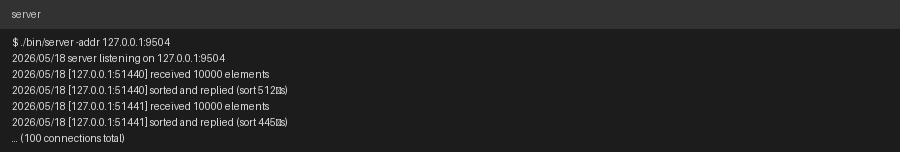
\includegraphics[width=0.92\linewidth]{../screenshots/server_log.png}
    \caption{Фрагмент журналу сервера}
\end{figure}

\begin{figure}[H]
    \centering
    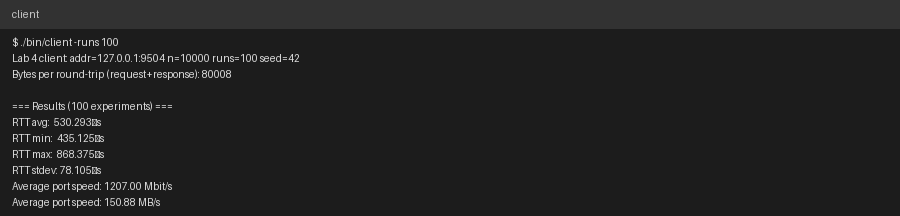
\includegraphics[width=0.92\linewidth]{../screenshots/client_results.png}
    \caption{Підсумок клієнта після 100 експериментів}
\end{figure}

\section{Висновки}

\begin{itemize}
    \item Реалізовано клієнт--серверну систему на Go з TCP і бінарним
    протоколом; усі 100~прогонів повернули коректно відсортовані масиви.
    \item На loopback домінує низька затримка; виміряна швидкість порту
    ($\approx$1.2~Гбіт/с) відображає ефективну передачу $\approx$80~КБ
    за $\approx$0.5~мс, включно з сортуванням на сервері ($\approx$0.4--0.8~мс).
    \item QuickSort на 10\,000 елементів не є вузьким місцем порівняно з
    накладними витратами встановлення TCP-з'єднання на кожній ітерації.
\end{itemize}

\end{document}
